\chapter{Result} \label{result}

\commento{\begin{itemize}
\item asymemtries on carbon.
\item expected rates on lead.
\item false asymmetriies result.
\item average of the asymmetries for the pmts.
\item confront with the theory.
\end{itemize}}

In this chapter we report the result obtained for the data-analysis. First we report the averaged asymmetries with and without subtracting the pmt offset. The sign of the asymmetry is given by the sign of the cross product between $\vec{k}$ incident electron and $\vec{k'}$ scattered electron. So we expect to see a positive sign for detector A and negative sign for detector B. From the asymmetry results, we can compute the factor $c$ as the ratio between the final asymmetries with and without subtracting the offset. The values can be directly confronted with the ones defined in \ref{Autocalib}. All the values are in reported in ppm.

\begin{table}[ht]
\centering
\subfloat[][\emph{Asimmetries, with offset not subtracted.} \label{table:NotCorrected}]{ 
\begin{tabular}{c|c|c}
\hline
 PMT   &   Average &   $\sigma$ \\
\hline
 B0    &    -19.92 &      7.7 \\
 B1    &    -19    &      7.8 \\
 B2    &    -23.42 &      8.7 \\
 A0    &     18.8  &      3.7 \\
 A1    &     16.05 &      3.4 \\
 A2    &     18.45 &      3.7 \\
 A3    &     19    &      4.2 \\
 A4    &     20.84 &      5   \\
 A5    &     22.83 &      4.9 \\
 A6    &     17.49 &      5.5 \\
 A7    &     19.24 &      6.6 \\
\hline
\end{tabular}} \qquad
\subfloat[][\emph{Asymmetries with offsets subtracted}\label{table:OffsetCorrected}]{
\begin{tabular}{c|c|c} 
\hline
 PMT   &   Average &   \sigma \\
\hline
 B0    &    -20.61 &      8   \\
 B1    &    -19.69 &      8   \\
 B2    &    -24.13 &      9   \\
 A0    &     24.55 &      4.2 \\
 A1    &     22.54 &      4.1 \\
 A2    &     24.37 &      4.3 \\
 A3    &     23.49 &      4.7 \\
 A4    &     24.21 &      5.4 \\
 A5    &     26.39 &      5.3 \\
 A6    &     19.82 &      5.9 \\
 A7    &     20.97 &      6.9 \\
\hline
\end{tabular}}
\qquad
\subfloat[][\emph{$c$ factor, as defined in \ref{eq:Systematic}} \label{table:Cfactor}]{
\begin{tabular}{c|c} 
\hline
 PMT   &        c \\
\hline
 B0    & 0.97 \\
 B1    & 0.96 \\
 B2    & 0.97 \\
 A0    & 0.77 \\
 A1    & 0.71 \\
 A2    & 0.76 \\
 A3    & 0.81 \\
 A4    & 0.86 \\
 A5    & 0.87 \\
 A6    & 0.88 \\
 A7    & 0.92 \\
\hline
\end{tabular}}
\caption{Averaged asymmetries over all the events. The values are corrected subtracting $\overline{A}_{I}$ and considering the effective polarization $p$ of the beam}
\end{table}

The asymmetries are shown with the corresponding errors in the following plot.
To Obtain a final asymmetry for detector A and B, the asymmetries for each plot are averaged using the formula:

\begin{equation}
\overline{A_{n}} = \sum_{i = 0}^{n_{PMT}} \dfrac{ w_{i} A_{i}}{\sum_{i = 0}^{n_{PMT}} w_{i}}
\end{equation}

This is a weighted mean, and $w_{i} = \frac{1}{\sigma^{2}_{i}}$. This formula must be used to take care of the different statistical error of the PMTs.

\begin{figure}[hbtp]
\centering
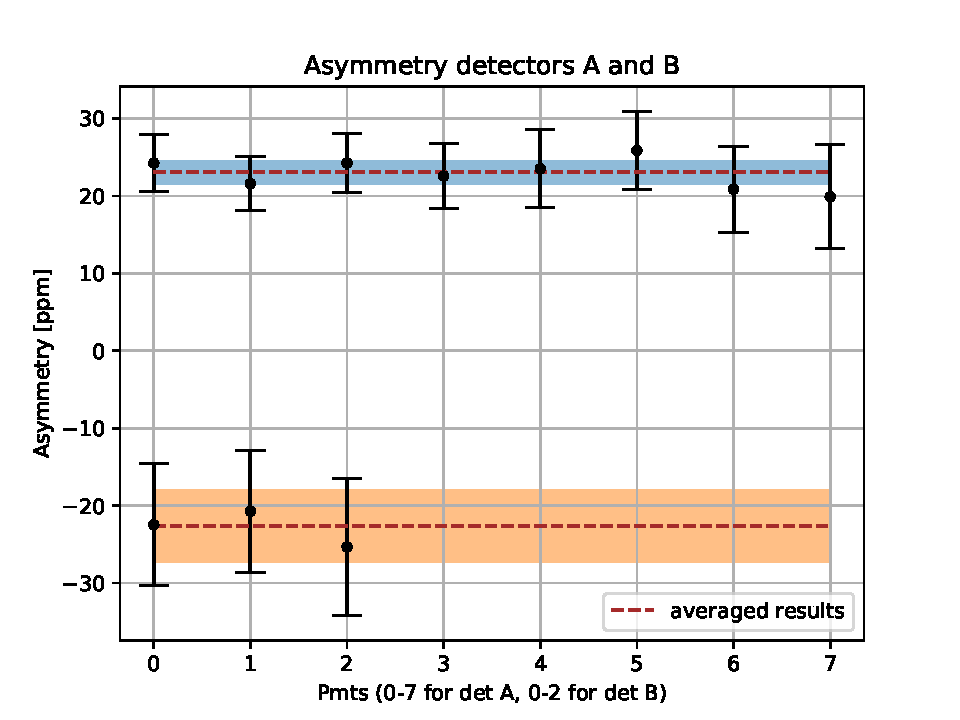
\includegraphics[width = 0.80\textwidth]{Analysis/Dataselection/FirstResult.pdf}
\caption{Plot of the PMTs asymmetries. The result are the average event per event, corrected by the beam asymmetry current 
$\overline{\delta I}$. }
\end{figure}

The overall results for the two detectors, without applying further cuts, are: 
\begin{itemize}
\item Asymmetry for detector A, $A_{A} =  23.6 \pm 1.7$ ppm.
\item Asymmetry for detector B, $A_{B} = -21 \pm 5$ ppm.
\end{itemize}

\section{data without polarization}

For the data without polarization, we report the result obtained from the fit:

\begin{table}[h]
\centering
\begin{tabular}{c|c|c|c|c|c}
\hline
 PMT   & An         & Ax        & Ay           & Ae         & $\chi _{reduced}$   \\
\hline
 A0    & -12 +/- 5  & 88 +/- 30 & 38 +/- 154   & -25 +/- 13 & 1.0 +/- 0.002   \\
 A1    & -9 +/- 5   & 44 +/- 29 & 57 +/- 149   & -23 +/- 13 & 1.0 +/- 0.002   \\
 A2    & -5 +/- 5   & 17 +/- 30 & 111 +/- 154  & -38 +/- 13 & 1.0 +/- 0.002   \\
 A3    & -7 +/- 6   & 47 +/- 32 & 85 +/- 163   & -51 +/- 14 & 1.0 +/- 0.002   \\
 A4    & -5 +/- 6   & 38 +/- 33 & 192 +/- 171  & -46 +/- 15 & 1.0 +/- 0.002   \\
 A5    & -4 +/- 6   & 67 +/- 34 & 177 +/- 173  & -52 +/- 15 & 1.0 +/- 0.002   \\
 A6    & -1 +/- 7   & 70 +/- 36 & -101 +/- 186 & -54 +/- 16 & 1.0 +/- 0.002   \\
 A7    & -1 +/- 7   & 25 +/- 41 & -494 +/- 209 & -41 +/- 18 & 1.0 +/- 0.002   \\
 B0    & -13 +/- 11 & 48 +/- 58 & -48 +/- 294  & 14 +/- 26  & 1.0 +/- 0.002   \\
 B1    & -11 +/- 11 & 51 +/- 58 & 44 +/- 295   & -3 +/- 26  & 1.0 +/- 0.002   \\
 B2    & -7 +/- 12  & 90 +/- 65 & -166 +/- 333 & -9 +/- 30  & 1.0 +/- 0.002   \\
\hline
\end{tabular}
\end{table}

The overall values are $-5 \pm 2$ for detector A and $-8 \pm 5$ for detector B.

\section{Best fit}
The result obtained from the linear fit of the asymmetries versus the beam parameters are reported here, together with the false asymmetry values. In this case the model is quite simple: only $X$, $Y$, $E$ are the beam parameters:

The result for detector A:
\begin{table}[h] 
\centering
\begin{tabular}{c|c|c|c|c|c}
\hline
 PMT   & $A_{n}$    & $A_{x}$          & $A_{y}$            & $A_{e}$         & $\chi^{2}_{reduced}$ \\
\hline
 A0    & 24 $\pm$ 4 & 67 $\pm$ 27  & -8 $\pm$ 135   & -22 $\pm$ 12 & 1.000 $\pm$ 0.002   \\
 A1    & 23 $\pm$ 4 & 9 $\pm$ 26   & -85 $\pm$ 130  & -10 $\pm$ 11 & 1.001 $\pm$ 0.002 \\
 A2    & 23 $\pm$ 4 & -12 $\pm$ 27 & -24 $\pm$ 134  & -21 $\pm$ 12 & 1.000 $\pm$ 0.002   \\
 A3    & 23 $\pm$ 5 & 14 $\pm$ 29  & -180 $\pm$ 142 & -31 $\pm$ 12 & 0.999 $\pm$ 0.002 \\
 A4    & 25 $\pm$ 5 & 50 $\pm$ 31  & -85 $\pm$ 151  & -26 $\pm$ 13 & 1.000 $\pm$ 0.002   \\
 A5    & 27 $\pm$ 5 & 31 $\pm$ 31  & 198 $\pm$ 152  & -37 $\pm$ 13 & 1.001 $\pm$ 0.002 \\
 A6    & 20 $\pm$ 5 & 7 $\pm$ 33   & 142 $\pm$ 164  & -31 $\pm$ 14 & 1.000 $\pm$ 0.002   \\
 A7    & 20 $\pm$ 6 & 6 $\pm$ 38   & 78 $\pm$ 184   & -14 $\pm$ 16 & 1.001 $\pm$ 0.002 \\
\hline
\end{tabular}
\caption{fit result with the linear model, for detector A.}
\label{tb:resultA}
\end{table}

the result for detector B:
\begin{table}[h]
\centering
\begin{tabular}{c|c|c|c|c|c}
\hline
 PMT   & An         & Bx         & By           & Be        & $\chi^{2}_{reduced}$\\
\hline
 B0    & -20 $\pm$ 8 & -59 $\pm$ 40 & -25 $\pm$ 187  & -14 $\pm$ 17  & 1.000 $\pm$ 0.002 \\
 B1    & -20 $\pm$ 8  & -64 $\pm$ 40 & 47 $\pm$ 188    & -22 $\pm$ 18 & 1.000 $\pm$ 0.002 \\
 B2    & -24 $\pm$ 9 & -65 $\pm$ 46 & -170 $\pm$ 211 & -61 $\pm$ 20 & 1.000 $\pm$ 0.002 \\
\hline
\end{tabular}
\caption{fit result with the linear model, for detector B.}
\end{table}

The final results of the \transv for the two detectors, for a $Q^{2} = \SI{0.04}{\giga \electronvolt \squared}$, computed with the weighted mean is:

\begin{table}[h]
\centering
\begin{tabular}{c|c}
\hline
 DETECTOR   & An    \\
\hline
 A          & 23.1 $\pm$ 1.7  \\
 B          & -21 $\pm$ 5   \\
\hline
\end{tabular}
\caption{Overall result for detector A and B.}
\end{table}
 

\chapter{Conclusion and outlook} \label{conclusion}

\commento{\begin{itemize}
\item outlook for the future experiments with lead.
\item mention the future experiment with Parity-violatin scattering.
\end{itemize}}